\section{Introduction}\label{introduction}

Technological advances have transformed how museums document, present and interpret their collections. Immersive experiences are realised through tools such as 3D printing and virtual reality \cite{allard2005use,Wachowiak01082009,RCM_2024_3D,Kuzminsky_LaserScan_2012,Schaich_3D_2007}. These technologies form a kind of experiential authenticity, enabling encounters that evoke the past's sensory, emotional, and intellectual essence \cite{trant_Auth_1999}. However, as Pine and Gilmore note \cite{pinegilmore_2007}, achieving authenticity requires museums to navigate the delicate balance between preservation and meaningful engagement—a challenge that is particularly evident in the case of historical musical instrument collections \cite{McAlpine2014}.

Musical instruments represent a peculiar fusion of form, function, and history. Their cultural value extends beyond their visual appeal to include the tactile and auditory dimensions of use \cite{Fritz2017}. Yet, preservation concerns often limit direct interaction, reducing these artefacts to static displays. This ``red velvet cord'' approach, as theorised by McAlpine \cite{McAlpine2014}, protects fragile mechanisms but diminishes the instruments’ functional identity, disconnecting visitors from the full richness of their historical and cultural context.

The Tagliavini Collection in Bologna \cite{Tagliavini2007}, renowned for its historical keyboard instruments, exemplifies this dilemma. With more than seventy early keyboard instruments, including many unique Renaissance Italian harpsichords, spinets and virginals, the collection stands out as a valuable resource for musicologists, organologists and musicians alike. Preserving the instruments' authenticity was the cornerstone of Ferdinando Tagliavini’s vision. This guiding principle led him to collect only playable instruments, or instruments which could be restored to playing condition after minimal intervention. 

However, the delicate mechanisms of these instruments and their historical significance mean they are only played under strict conditions—typically during concerts or by experienced performers with special permission from the curator. 
To enhance accessibility and engagement, the museum commissioned the replica (Figure \ref{fig:teaser}) of a historical keyboard built in the tradition of the Italian Renaissance and is the subject of this paper.
The keyboard, which museum visitors can use without special permission, presents two choirs of muted strings and can generate MIDI messages. The interface is currently connected to a software sampler loaded with the Spitfire sample library, though the ultimate goal is to use samples of instruments from the collection. Visitors to the museum are invited to play the interface and listen through a pair of headphones. This work outlines the technological aspects of interface's construction and offers reflections on its role within the Tagliavini Collection and potential application within the wider musical instrument museum context. 
% The paper outlines the design and motivations behind this replica keyboard interface.


\section{Related Work and Motivations}\label{related-work}


Museums face a constant tension between accessibility and preservation, restricting how visitors can interact with collections \cite{Templeton2018, McAlpine2014}. For musical instrument museums, these challenges are compounded by the difficulty of preserving historical instruments in a playable condition \cite{McAlpine2014}. The instruments' inherent fragility and gradual decay inevitably result in a point where they can no longer be played, even when collections adhere to the strictest conservation protocols \cite{NYT_strad}. A marked cultural change has taken place in recent decades, shifting the focus from the playability of the originals to their conservation. Karp \cite{Karp1979,Karp1985} advocates for a deeper understanding of musical instruments so that enough knowledge is generated to make them as ``copyable'' as possible.

McAlpine discusses a case similar to the Tagliavini collection in his examination of the Benton Fletcher Collection at National Trust Fenton House \cite{McAlpine2014}. When these instruments were donated, Benton Fletcher stipulated that they remain playable and should continue to be maintained for tuition and public performance. A large sampling campaign was conducted, and a custom MIDI interface was designed to fulfil this requirement while preserving the original instruments' integrity. The MIDI controller, comprising two commercially available keyboards mimicking the two-manual harpsichord layout, was used by visitors to trigger the instrument samples recorded with tailored strategies for each. However, user tests identified a limitation: the commercially available weighted keys failed to provide an authentic sense of interacting with a historical keyboard \cite{McAlpine2014}. 

On the other hand, the ``Tromba Moderna'' project \cite{Baldwin2016}, a previous NIME initiative, approached the issue of musical heritage playability by recreating and augmenting a replica of a historical tromba marina. A piezo transducer was connected to a sound synthesis engine and a driver within the instrument to simulate the expected vibrations of a historical tromba marina. 

\begin{figure}
  \centering
  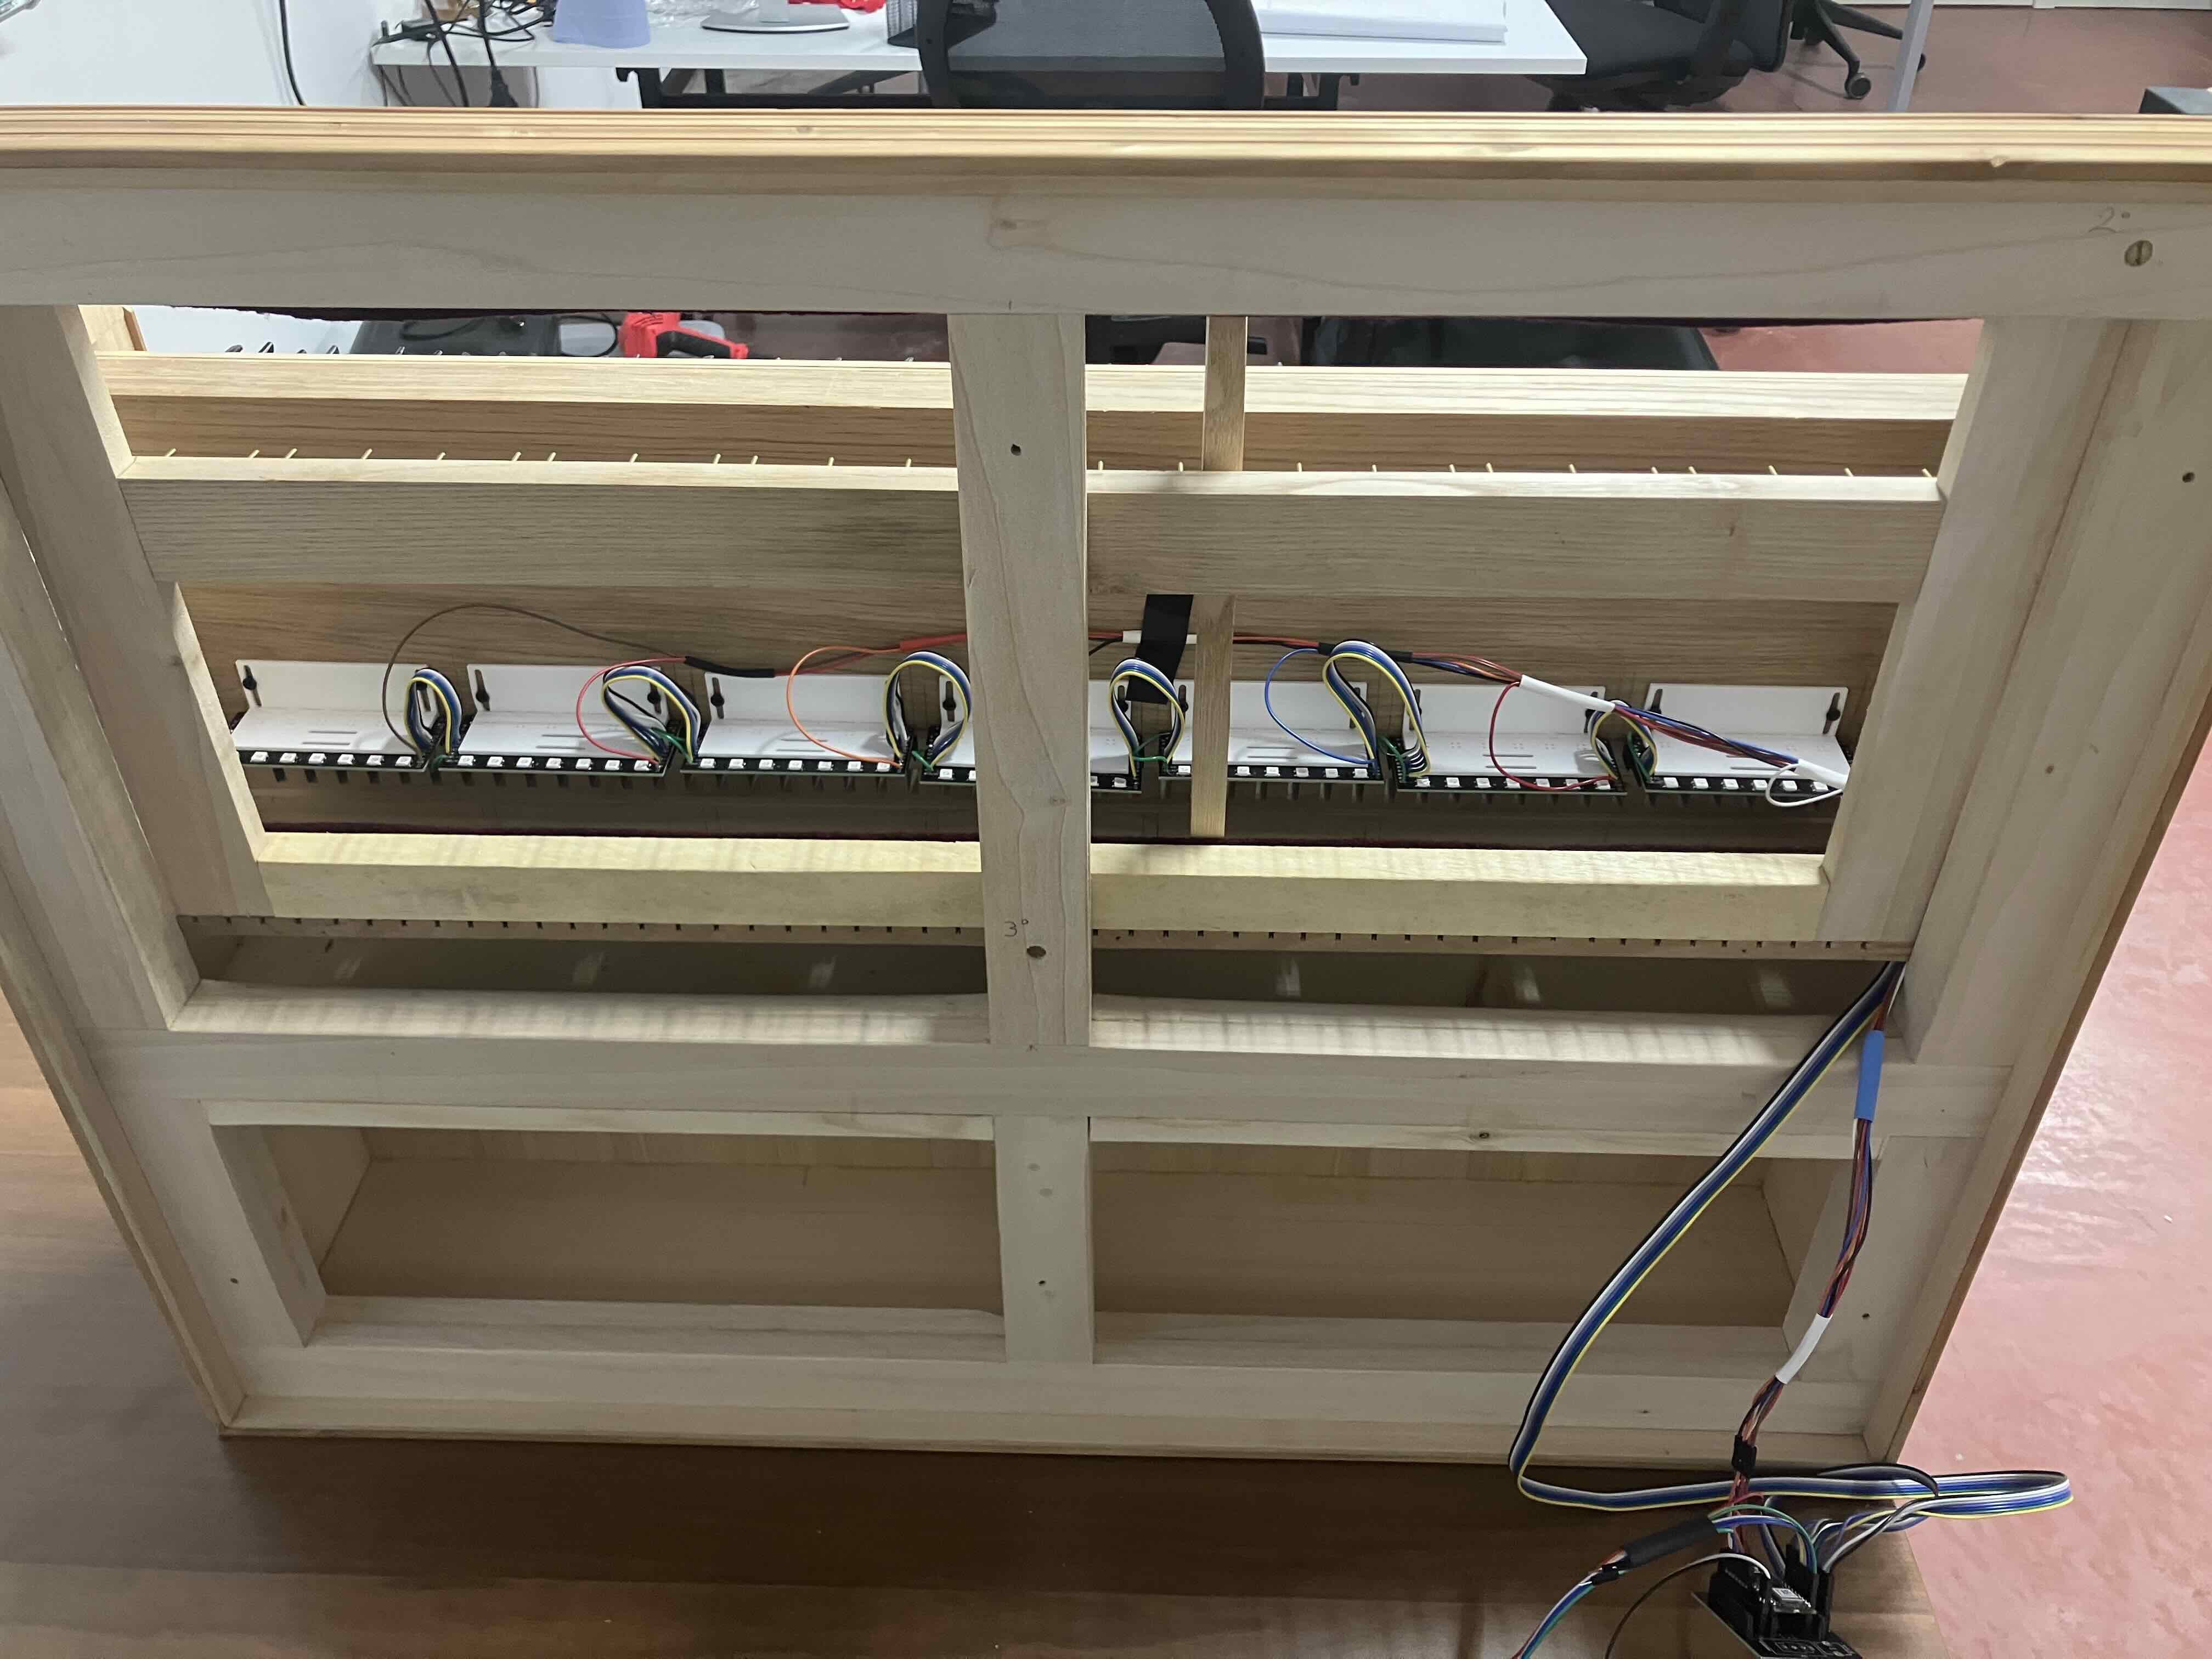
\includegraphics[width=\linewidth]{src/images/49-key-bottom-sensors-no-keys.jpg} 
  \caption{Underside of the full model keyboard, showing two chambers: the front chamber (top) and the rear chamber (bottom).} 
  \Description{} 
  \label{fig:49-key-bottom}
\end{figure}

\begin{figure}
    \centering    
    \includegraphics[width=\linewidth]{src/images/3-key-side.png}
    \caption{3-Key Model Harpsichord Mechanism acquired from San Colombano, Bologna, 2023}
    \label{fig:3key}
\end{figure}

\begin{figure}  
  \centering
  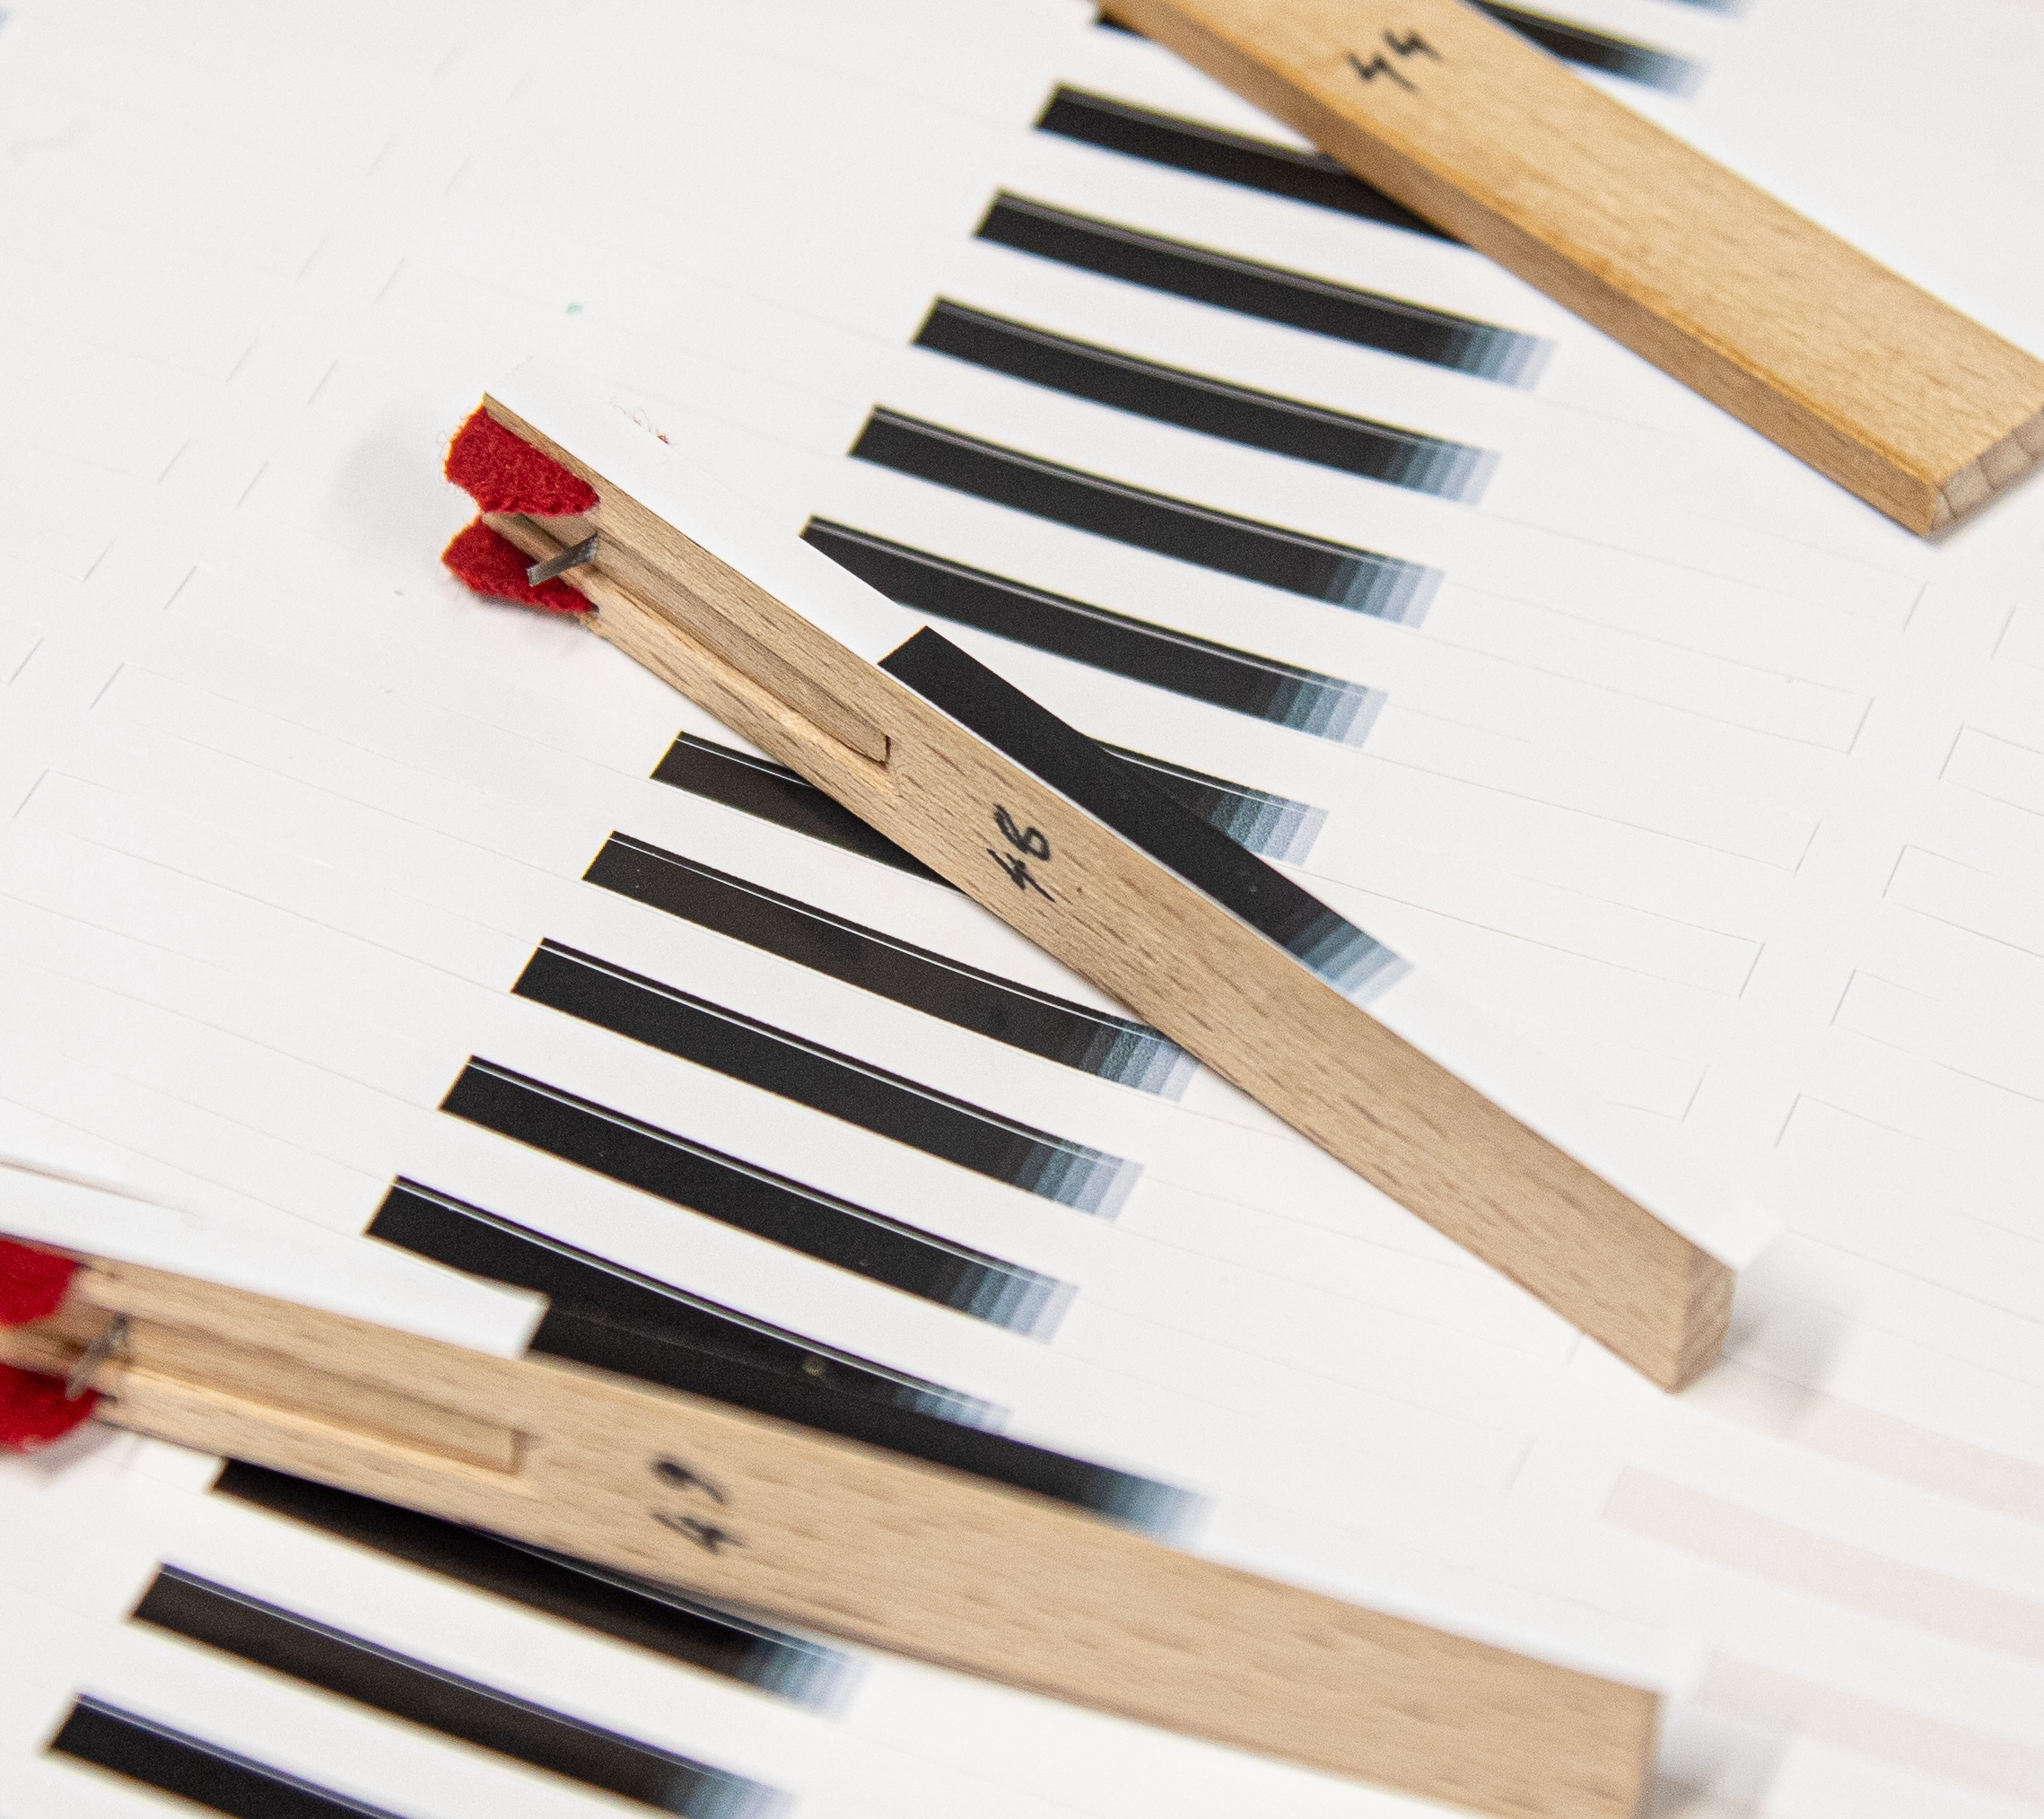
\includegraphics[width=\linewidth]{src/images/tagging-jacks-3.jpg} 
  \caption{Gradient stickers applied to the side of the jack body. The coarse gradient scale was selected to maximise signal excursion while preserving signal readout stability.}
  \Description{} 
  \label{fig:jack-tags}
\end{figure}

\begin{figure}  
  \centering
  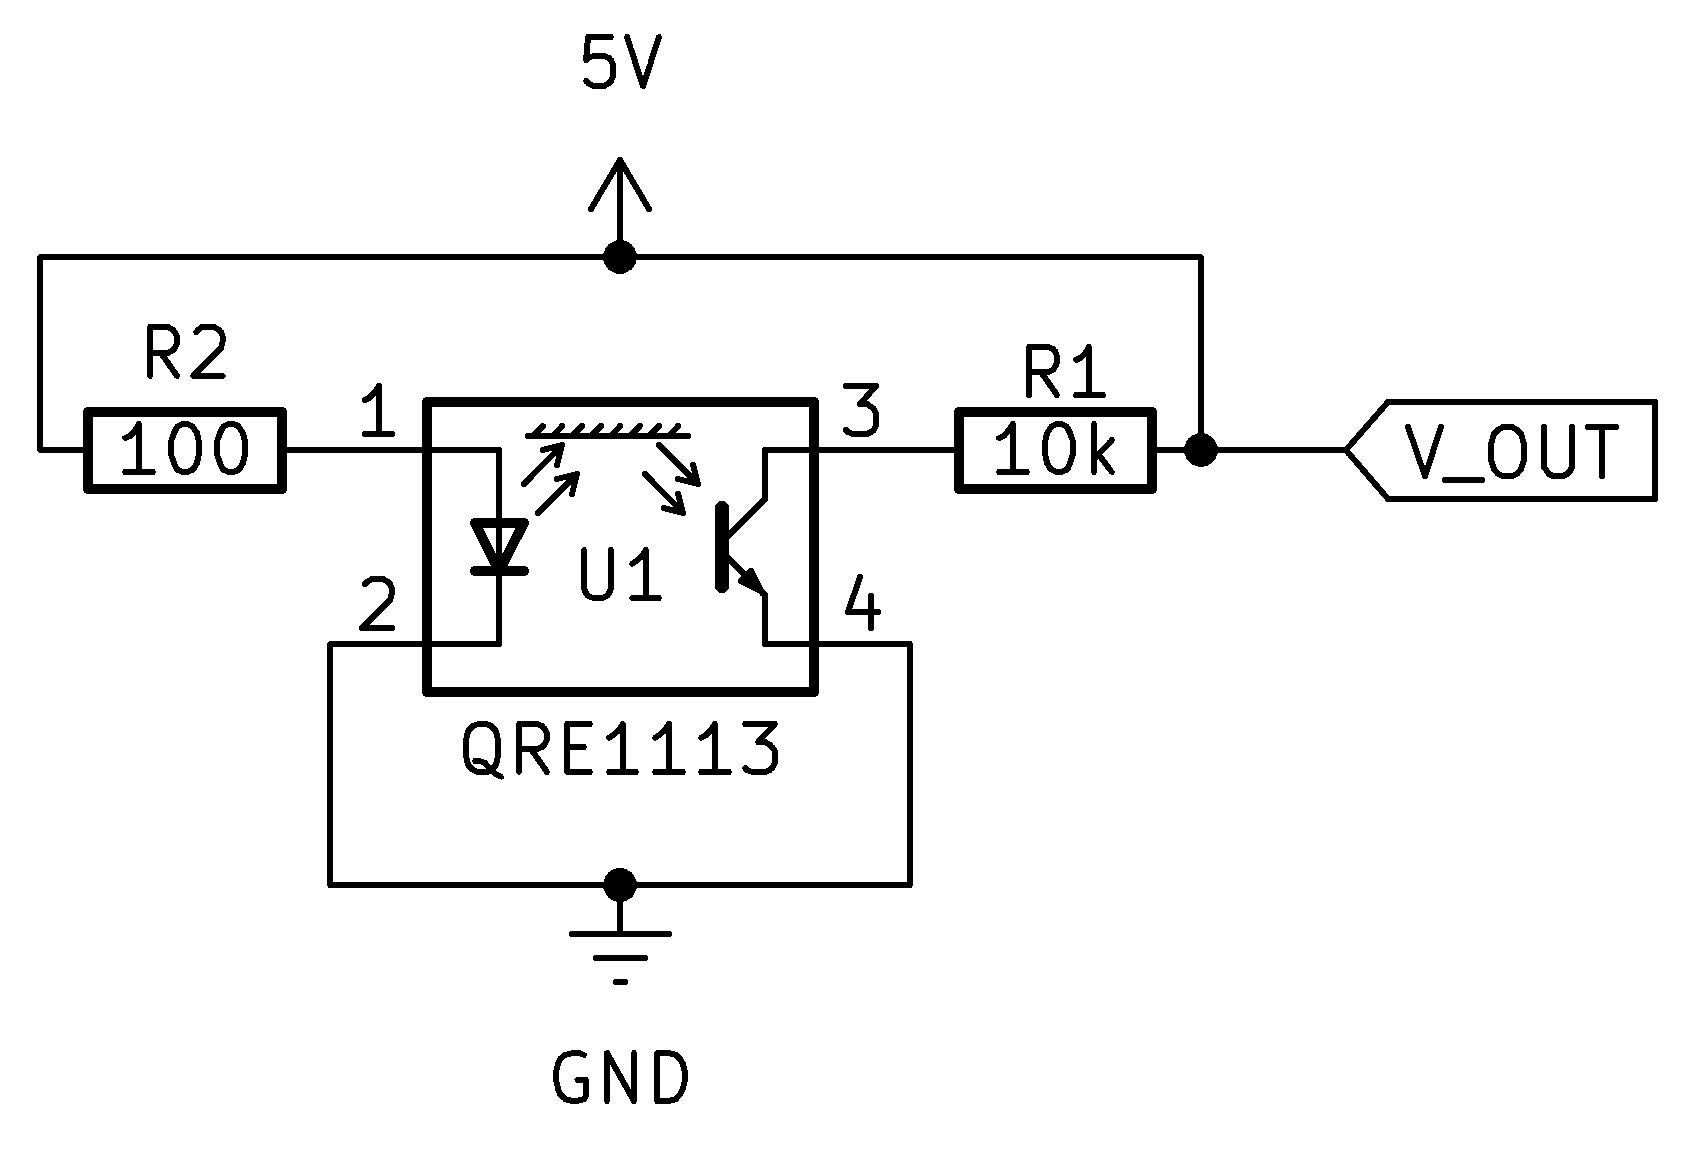
\includegraphics[width=\linewidth]{src/images/simple-schematic-bw-.jpg} 
  \caption{Optical sensor in a simple voltage divider circuit. \texttt{V\_OUT} is routed to one of 8 channels on the CD4051BE multiplexer}
  \Description{} 
  \label{fig:simple-schematic}
\end{figure}

\begin{figure}
    \centering
    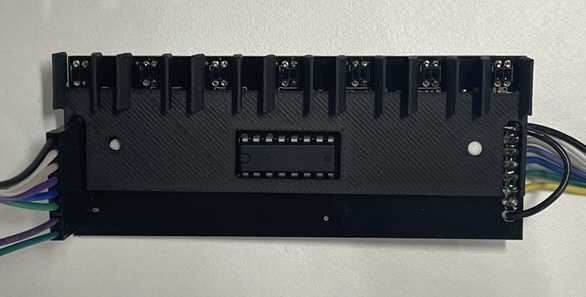
\includegraphics[width=\linewidth]{src/images/sensor-board-w-baffles.jpeg}
    \\
    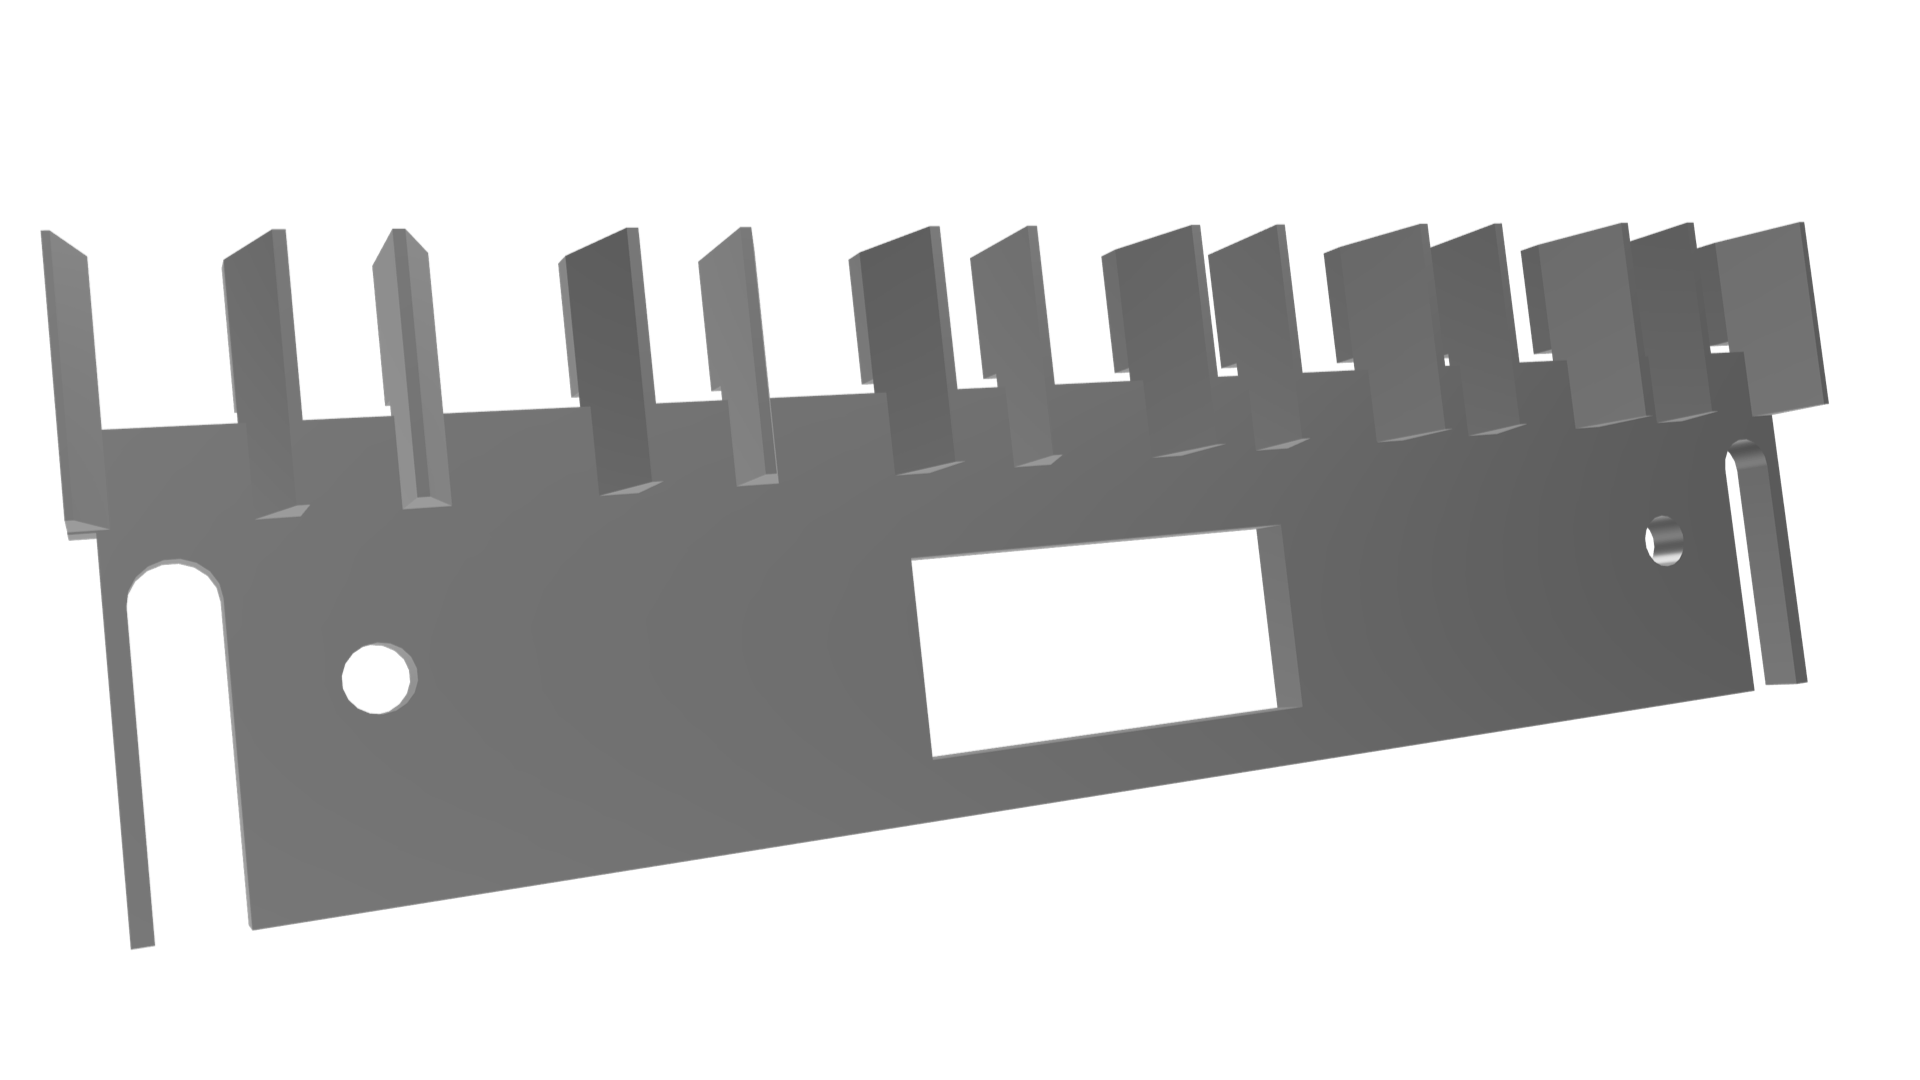
\includegraphics[width=\linewidth]{src/images/baffles.png}
    \caption{Baffles designed to prevent cross-talk between adjacent sensors.}
    \Description{}
    \label{fig:baffles}
\end{figure}
\subsection{Controller Board}\label{controller-board}

\begin{figure}
\centering
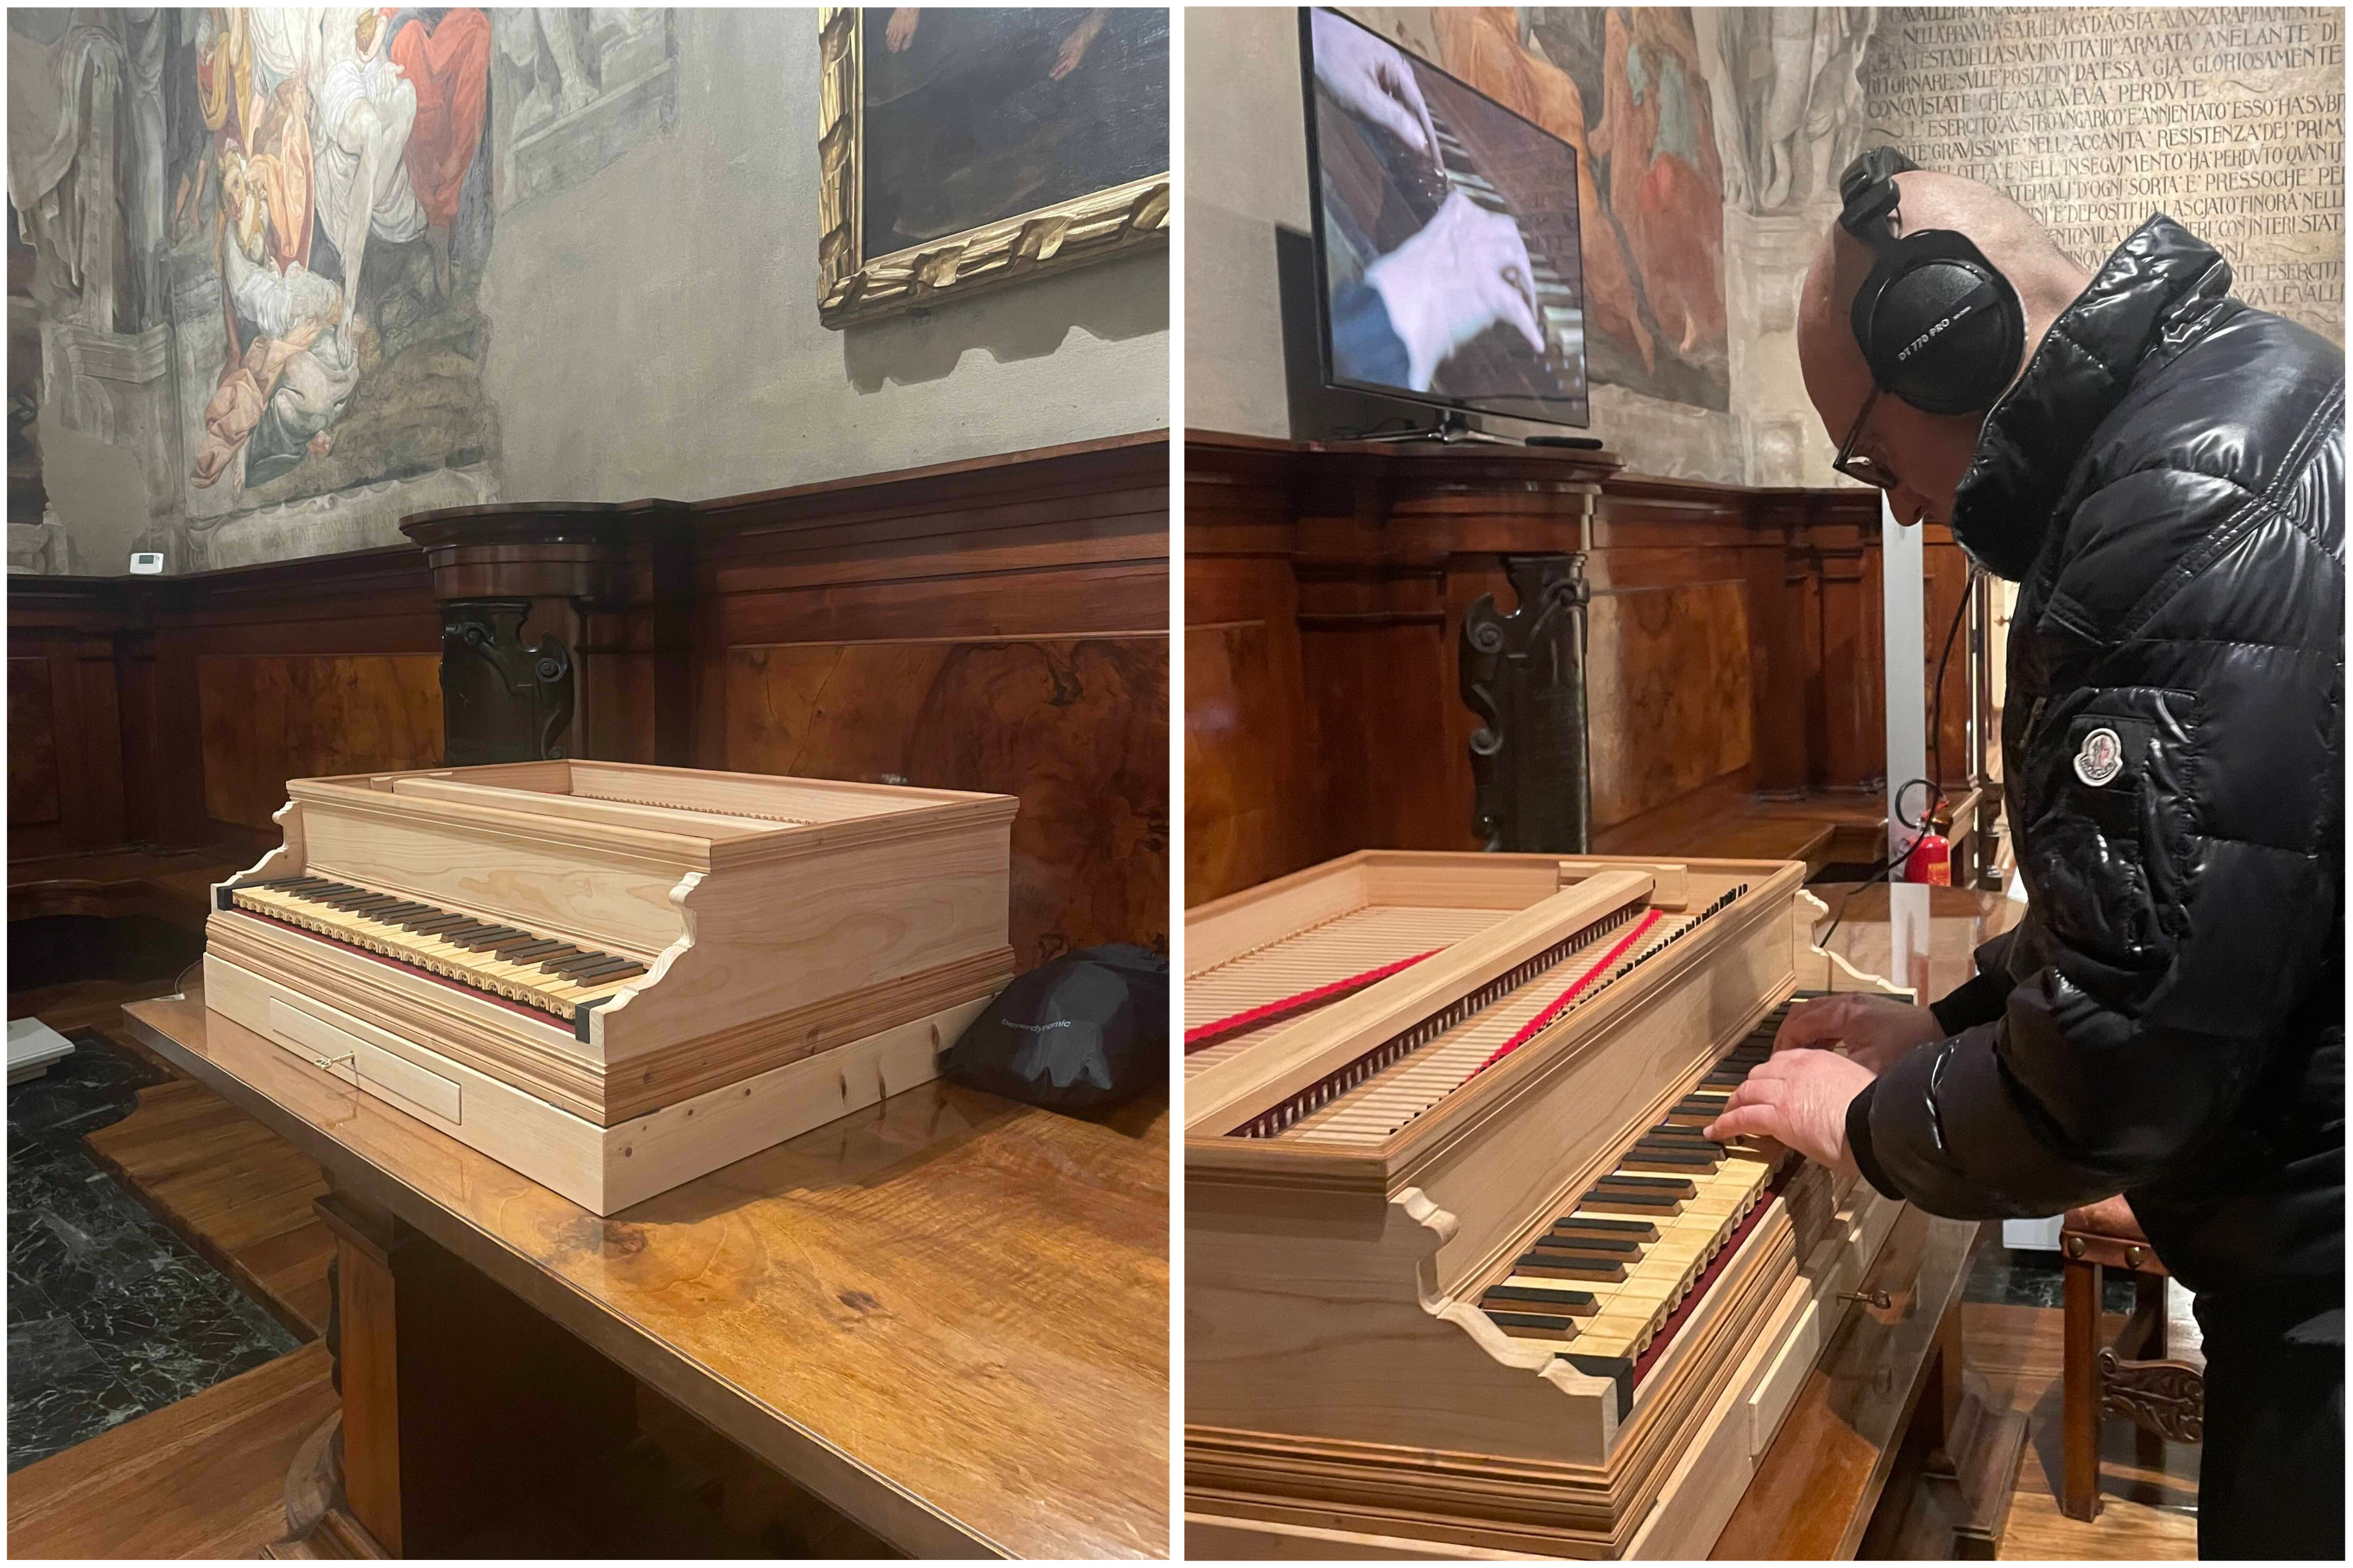
\includegraphics[width = \linewidth]{src/images/keyboardMuseum.JPEG}
\caption{The keyboard installed in the \emph{Oratory} at San Colombano, and a user wearing headphones playing it.}
\label{fig:oratory}
\end{figure}



The keyboard presented here inherits some aspects from the Tromba Moderna project. The project aims to offer a tool to enhance the fruition of the Tagliavini collection while retaining a form of continuity with historical instrument-building traditions. However, the electronics hidden inside the interface are not intended to augment or disrupt the tactile feedback; rather, they serve as the silent and invisible link between the mechanical and the digital realms. 
The optical sensing technique for the keyboard is adapted from a similar project on the piano by McPherson \cite{McPherson2013}. 
Thus, whether the interface proposed here is a \emph{new} musical interface is subject to discussion, particularly regarding the keyboard's tactile response designed to adhere to longstanding harpsichord building traditions. This work complements and follows up on previous reflections within the NIME community, emphasising the \emph{O} in NIME \cite{Masu_NIME_2023}. The intended use of the keyboard through meaningful interaction with a museum exhibit is where the novelty of this work lies, rather than solely in its technological development. Relying on previous NIMEs, this project extends the longevity of the results beyond the scope envisaged in the original works, enhancing their sustainability, as discussed by Masu \emph{et al.} \cite{Masu_NIME_2023}.

Besides enhancing the visitor experience, future design iterations will serve as a research tool to explore the unique characteristics of the harpsichord and its impact on performance through the \anon{ERC-funded NEMUS} project \anon{\cite{NEMUS}}, aiming to virtually reproduce the sound of historical keyboard instruments, and upcoming projects such as Rem@ke \cite{remake1} investigating embodied relationships between instrument and performer.

\begin{figure*}
\centering
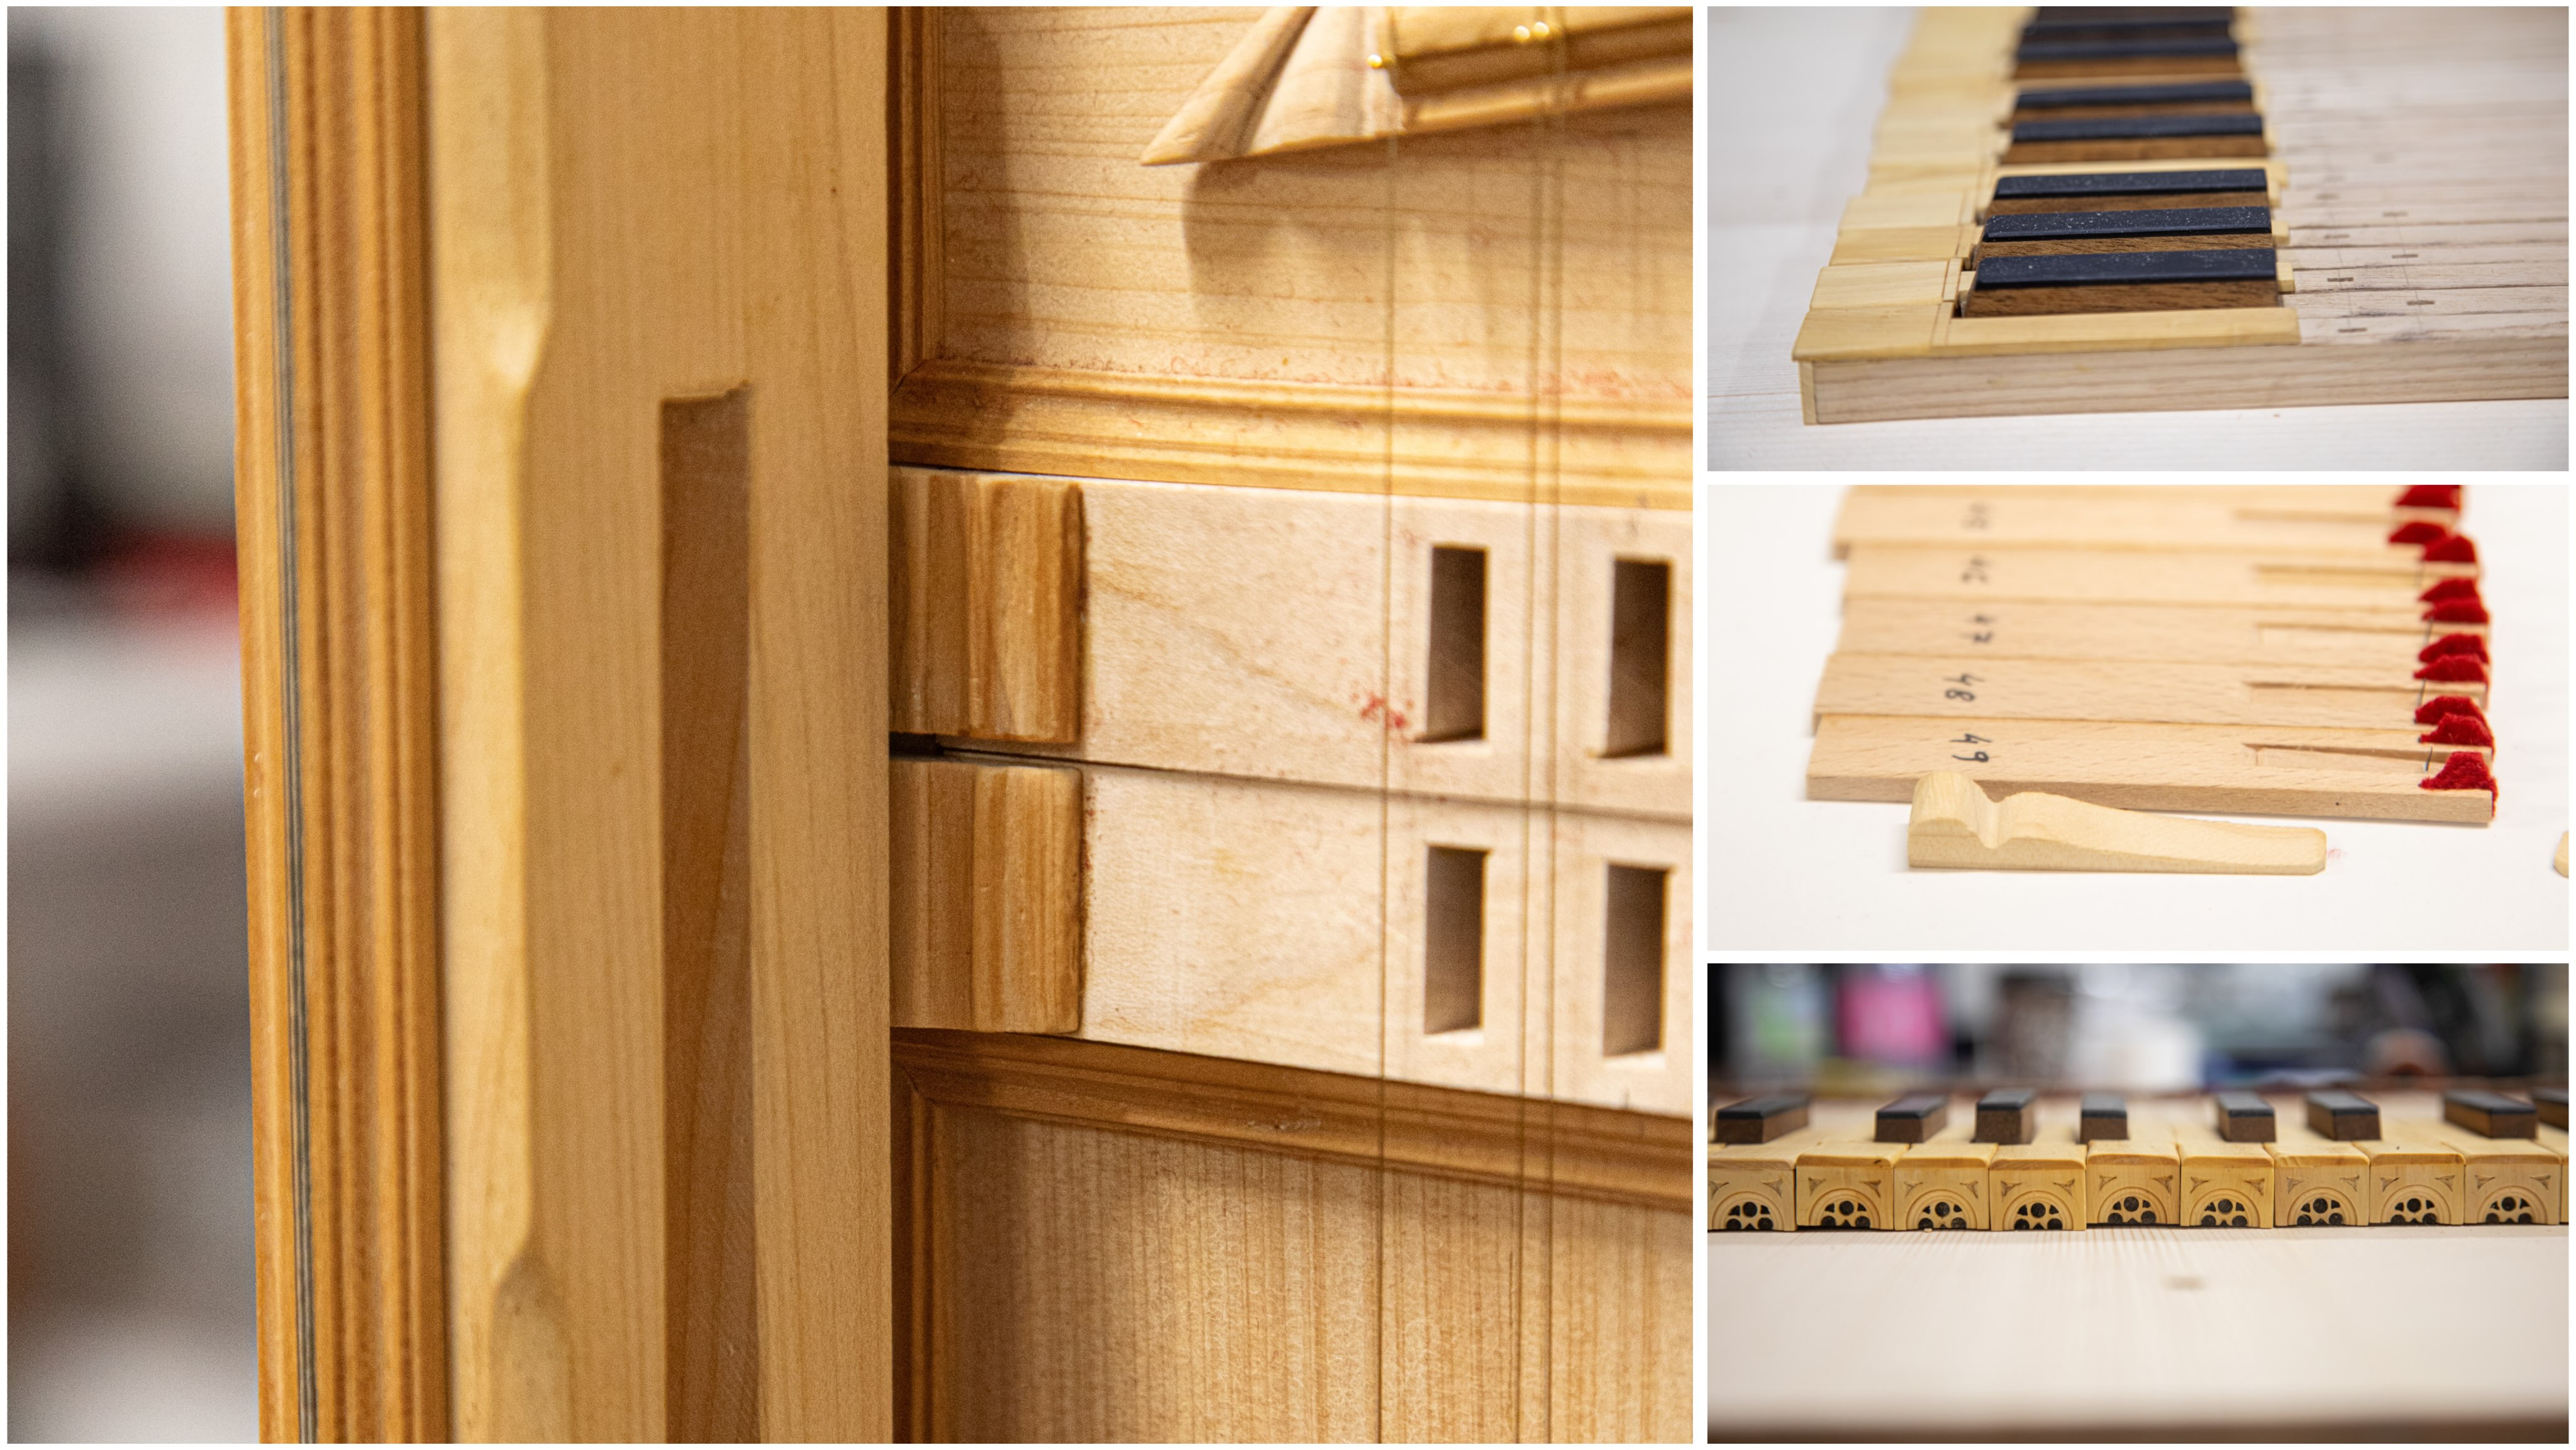
\includegraphics[width=0.8\linewidth]{src/images/details.jpg}
\caption{Details of the replica, including the key slots and sides, keys, and jacks with seagull plectra.}\label{fig:details}
\end{figure*}

\section{Design Principles}\label{design}

The design of the augmented replica keyboard for the Tagliavini Collection was guided by three principal constraints stipulated by the museum:
\begin{itemize}
\item \emph{No visible electronics}. To preserve the visual integrity of the exhibit, all electronic components had to remain concealed except for a pair of headphones and a small display for audio parameter adjustments.
\item \emph{Robustness and reliability}. The system needed to accommodate frequent use by museum visitors and allow for straightforward maintenance by staff without requiring specialised technical expertise.
\item \emph{Faithfulness}. The keyboard mechanism ensured fidelity to its authentic operation, keeping artefacts to a minimum. 
\end{itemize}
These constraints demanded a non-invasive, robust design that was respectful of the historical authenticity of the instruments. The requirement for faithfulness to the original mechanism immediately ruled out a mechanical design reliant on electromechanical actuators, as in previous works on piano haptics \cite{Timmermans2020,Gillespie1996}. While actuators can generate considerable force, they cannot replicate the wideband signals characteristic of the harpsichord's sharp and responsive haptics (A REFERENCE WOULD BE GOOD HERE, ANY IDEAS?), which differ significantly from a piano.

%\subsection{Summary of the Finalised Design}

The final design, visible in Figures \ref{fig:teaser} and \ref{fig:details}, is a 49-key harpsichord keyboard replica equipped with an optical sensor, whose voltage output depends on the amount of light reflected by sensor surface. In this case, a sensor surface is a grey-scale gradient printed on a vinyl sticker and applied to the side of each jack (Figure \ref{fig:jack-tags}). 

    
\subsubsection{Alternative}
\textcolor{red}{
The final design, visible in Figures \ref{fig:teaser} and \ref{fig:details}, is a 49-key two-register harpsichord keyboard replica.
The keyboard was consciously chosen to mimic that of the original XVI century Italian harpsichords. This design decision was made in order to use the propensity humans have to being influenced by visual components when musical making judgements \cite{Tsay2013} to our advantage. It is especially true with respect to musical instruments as the studies by Fritz \emph{et al}\cite{Fritz2012, Fritz2014, Fritz2017} have clearly shown. Rather than avoiding this effect we have chosen instead to utilise it. This `musical instrument McGurk effect' is in part the reason behind hiding the electronics out of sight. 
The aesthetics of the interface make it more likely that the interface be accepted on the same terms as an `authentic' musical instrument. With all the work into modelling and recreating piano action \cite{Cadoz1990, Gillespie1996, Timmermans2020} it is possible the visual component my provide the necessary push of acceptance similar to that which influences our judgment on performance \cite{Tsay2013}. 
% Such an effect is invaluable if visitors are expected to engage with the interface on an equal footing as the historic instruments that neighbour it in the museum.
% The keyboard in not merely a facsimile of a harpsichord, but rather by being equipped with optical sensors, it can provide modes of expression with a digital instrument which would otherwise be inaccessible to its analogue sibling. 
The optical sensors are wired in a voltage divider configuration (Figure \ref{fig:simple-schematic}) whose voltage output depends on the amount of light reflected by sensor surface. In this case, a sensor surface is a grey-scale gradient printed on a vinyl sticker and applied to the side of each jack (Figure \ref{fig:jack-tags}). Though the current configuration simply sends MIDI note on and off at passing a threshold, the displacement of all jacks is available continuously.
The staggering of pluck point of the jack means that there are two very distinct tactile `anchors' along the key dip. A combination of string tension, quill voicing and jack staggering contribute to the overall `weight' of the action, with each key differing from the low to the high octaves \cite{Veroli2012}. Such tactile expectations provide fertile opportunities for extending the expressive capabilities of the interface. The current sensor system should for recording of traditional use and identify where those opportunities for new expression lie \cite{McPherson2013-2}. 
}

% "When working with an established interface like the keyboard, it is particularly important that new mappings do not interfere with familiar technique (McPherson, Gierakowski, and Stark 2013). The Space Between the Notes: Adding Expressive Pitch Control to the Piano Keyboard"

A modular system of printed circuit boards (PCBs) was designed to manage the sensors and process their output. The system uses 49 optical sensors which are distributed across seven boards that contain 7 sensors each. The PCBs were secured to the underside of wrest plank and above the keys (Figure \ref{fig:49-key-bottom}), allowing them to be adjusted during installation. Ribbon cables connected the PCBs, providing flexibility during assembly while maintaining a compact form factor. Additional modifications, including baffles and adhesive improvements, were made to optimise the reliability of the sensor system during calibration and use.

The project expanded upon earlier NIME research on generating MIDI messages from piano keystrokes \cite{McPherson2013}, adapting it to address the specific characteristics of harpsichords. Whereas the previous design emphasised continuous gesture tracking, this implementation required discrete key-triggered data to align with the needs of MIDI-triggered audio playback. 

\subsection{Project Deployment}
A further objective, set forth by the authors, was to ensure accessibility and reproducibility by committing to an open source approach for all outputs of the project. The commitment to open sourcing encompassed all aspects of the system, including hardware schematics, firmware, and calibration data. Cost-effectiveness was also a central consideration. The system was initially developed for a 3-key prototype, shown in Figure \ref{fig:3key}, and successfully scaled to 49 keys without significant increases in cost or complexity. Specifically, the system was designed to be easily assembled using resources typically available in a university-managed maker space.

Components, such as QRE1113 optical sensors and CD4051BE multiplexers, are widely available from commercial resellers, while the modular PCB design ensures easy replication and maintenance.

The Arduino Nano 33 BLE was chosen as the core microcontroller for its compatibility with open source tools and ability to support both USB and BLE MIDI. Ferroelectric RAM (FRAM) was employed for data storage since it offers an economical yet robust solution for preserving calibration settings across power cycles. Calibration workflows were optimised using the Arduino IDE’s serial plotter and open source MIDI Monitor software, reducing reliance on proprietary tools and simplifying the process for users. 

\begin{anonsuppress}
Reference repositories for this project can be found here:

    \begin{itemize}
        \item 
        \emph{Firmware}: \anon{\url{https://github.com/Nemus-Project/harpsichord-interface-firmware}}
        \item 
        \emph{PCB CAD}: \anon{\url{https://github.com/Nemus-Project/harpsichord-interface-cad}}
        \item 
        \emph{Interface Models}: \anon{\url{https://github.com/Nemus-Project/harpsichord-interface-models}}
    \end{itemize}
\end{anonsuppress}
% FILL OUT AS APPROPRIATE (and anonymise).



\subsection{Materials and Construction}

The keyboard was designed to replicate the tactile and aesthetic sensations of playing an antique Italian harpsichord. Traditional materials were used, including walnut for the wrest plank, chestnut for the key levers, boxwood and ebony for key covers, and cypress for the case and soundboard. The 98 jacks were made from beech, fitted with brass springs and natural seagull feather plectra. The design was inspired by Venetian harpsichords, particularly the 1547 Alessandro Trasuntino harpsichord at the San Colombano Museum. An exception was made for the short octave --- the assigning of common keys in the first octave over a chromatic scale --- typically found in Italian harpsichords: this was replaced by a standard octave layout to more easily accommodate the interaction with commercial sample libraries. 

The rectangular poplar frame also deviates from the traditional logarithmic form to allow for the installation of the electronic sensors, as visible in Figure \ref{fig:49-key-bottom}, without compromising the visual or tactile authenticity. Two string choirs, crafted from yellow brass wire and anchored with wrought iron pins, were tensioned to replicate authentic plucking resistance. Felt strips were added to dampen vibrations. The result is an interface that combines the mechanical action of keys with synthetic sound generation, preserving a real harpsichord's tactile qualities.


\section{Hardware Design}\label{hardware-design}

Figure \ref{fig:system-block-diagram} shows a block diagram of the finalised hardware setup. The system evolved through iterative prototyping, beginning with simple threshold-based testing and ending in a fully functional multi-sensor interface capable of triggering MIDI events. 

\subsection{Prototype Stage}

The initial stage of development focused on testing whether sensor data could reliably trigger MIDI playback. Modifying an existing harpsichord for testing was considered but ultimately discarded due to significant internal measurement and layout discrepancies. Instead, a custom 3-key harpsichord mechanism (Figure \ref{fig:3key}) was acquired from the museum and used as a foundation for prototyping. This approach followed a methodology similar to that used in Timmermans \emph{et al.}'s Haptic Key project \cite{Timmermans2020}, since the 3-key model enabled iterative testing of individual components, including sensor placement, signal processing, and mechanical tolerances, before upscaling. 





%\subsection{Sensor Criteria}\label{sensor-criteria}

The following criteria were established to guide sensor selection and integration to make the system suitable for a museum context:

\begin{itemize}
    \item \emph{Non-invasiveness.} No remarkable modifications were allowed on the harpsichord mechanics, particularly on all the visible parts.
    \item \emph{Low Latency.} The time required to process a single iteration of all sensor data should remain under 10 ms, with an upper limit of 25 ms deemed acceptable. Empirical criteria found in previous studies \cite{Jack2016} was used as a guide.
    \item \emph{Reliability:} Sensor data should be dependable and consistent, with interference from anything external to the jack movement being absent or negligible.
    \item \emph{Scalability.} The design needed to scale in both cost and time in order to be adaptable from a 3-key prototype (figure \ref{fig:3key}) up to the 49 keys of the final design.
    % \item \emph{Expandability.} The system should accommodate future functionality, such as additional MIDI parameters or data visualisation.
\end{itemize}

The hardware was designed to make assembly possible in standard maker spaces.  

\subsection{Sensor Board Design}\label{sensor-board}

\begin{figure*}
    \centering
    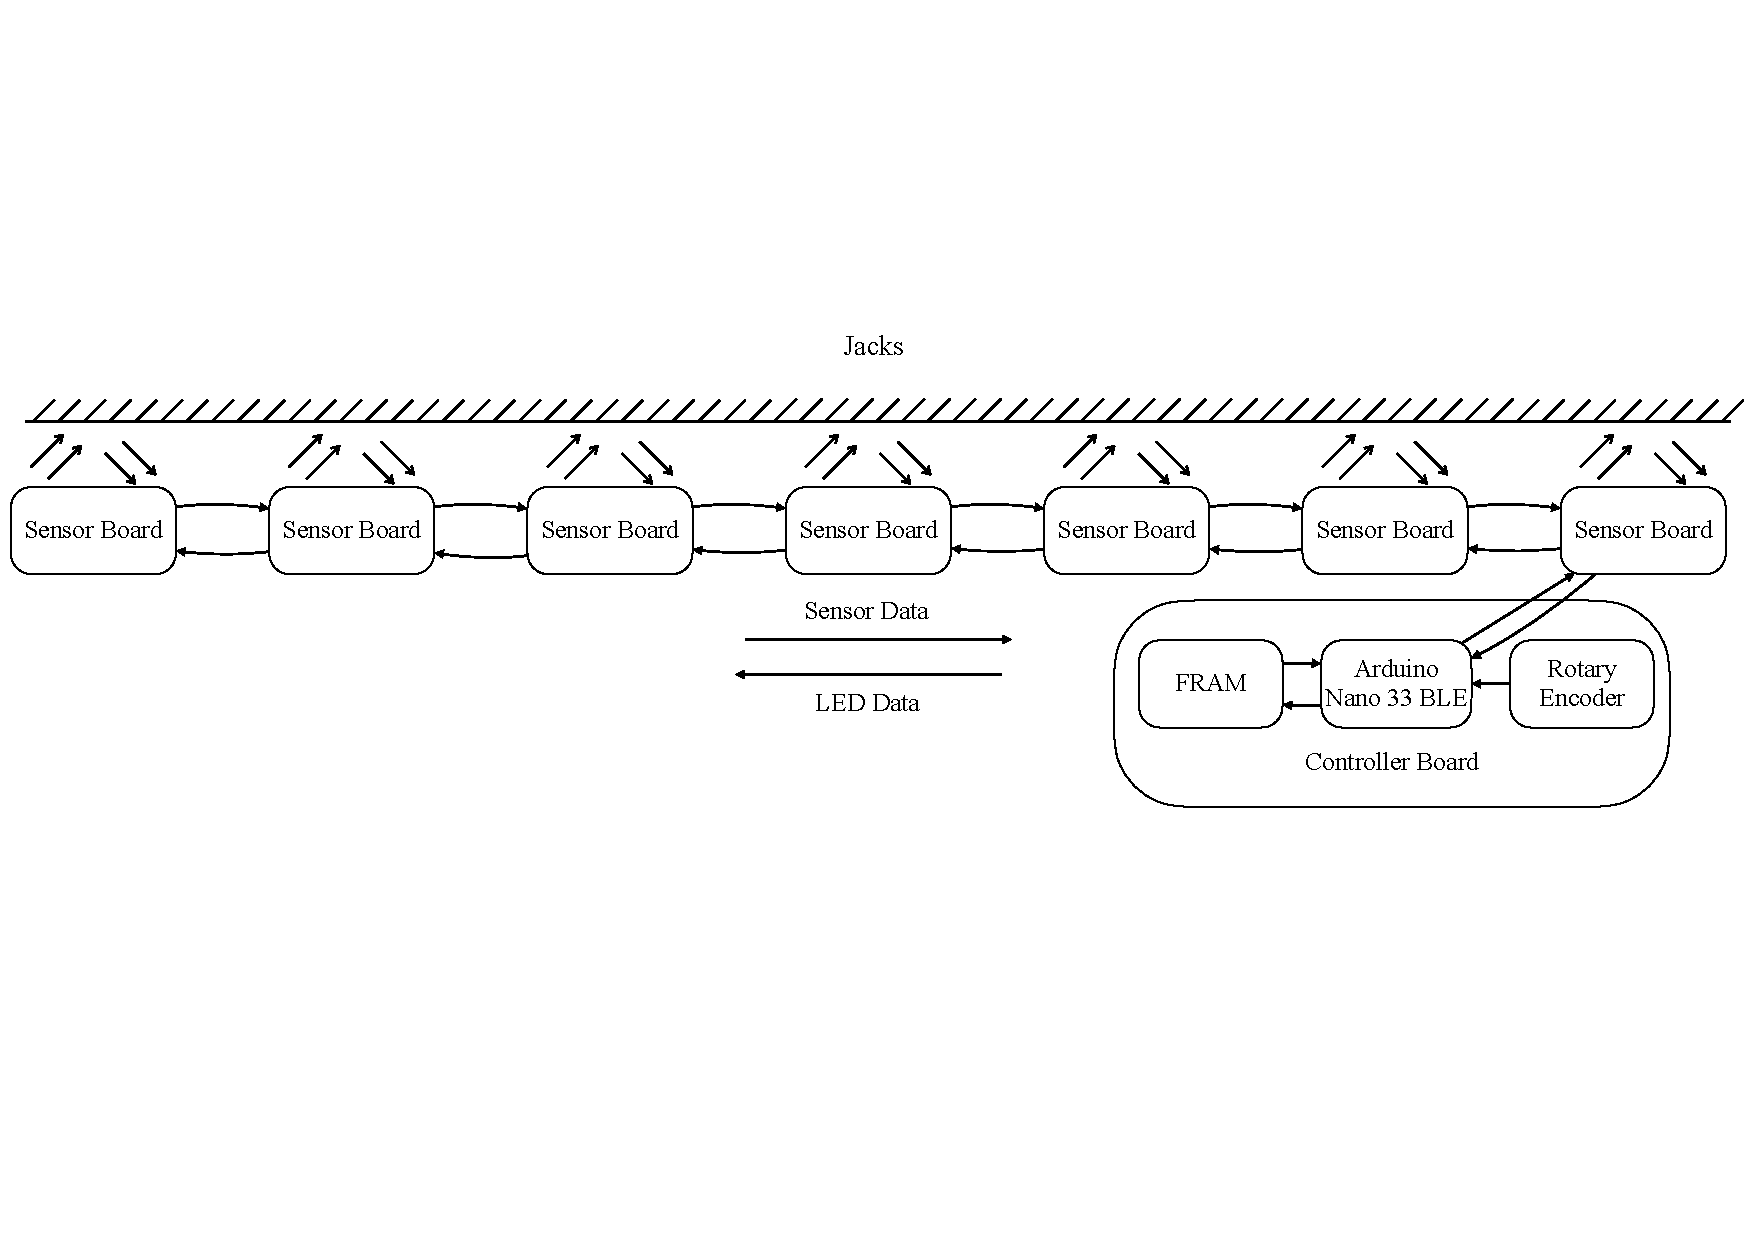
\includegraphics[width=\linewidth]{src/images/block-diagram.pdf}
    \caption{Block diagram of PCB connections. Sensor and LED are routed through each sensor PCB}
    \label{fig:system-block-diagram}
\end{figure*}

The final sensor system utilised QRE1113 optical sensors, known for their small form factor, low cost, and suitability for short-range distance detection \cite{McPherson2013, McPherson2019}. The sensors were distributed across seven printed circuit boards, each responsible for seven keys. Each PCB contained the following components:

\begin{itemize}
    \item 7 QRE1113 optical sensors.
    \item 7 100 $\Omega$ resistors and 7 10 k$\Omega$ resistors (later reduced to one resistor per board).
    \item 1 Texas Instruments CD4051BE multiplexer for signal aggregation.
\end{itemize}

The optical sensors detect infrared light reflected from nearby surfaces, as per Figure \ref{fig:simple-schematic}. The gradient stickers affixed to each jack provided a consistent reflective surface for the sensors (Figure \ref{fig:jack-tags}), which were used to track jack displacement precisely. 


3D-printed baffles were installed on the PCBs to eliminate cross-talk between adjacent sensors, as per Figure \ref{fig:baffles}. These baffles, fabricated from dark-pigmented PLA, ensured that infrared reflections from neighbouring jacks did not interfere with sensor readings. Testing confirmed that this measure significantly improved data reliability.



The controller board, designed around the Arduino Nano format, was the central hub for processing sensor data and triggering MIDI messages. The in addition to solder terminals for sensor board channels, the controller board contained of:

\begin{itemize}
    \item 1 Arduino Nano 33 IoT
    \item 1 Fujitsu MB85RS64 SPI FRAM chip
    \item 1 EC11 combined rotary encoder and tactile switch
    % \item 1 DFROBOT DFR0785 Tactile Switch
\end{itemize}


The Arduino Nano was selected for its compact form factor and native USB support. The 33 BLE variationof the Nano had the additional benefit in its ability to be programmed as BLE MIDI device.  Initial iterations of the controller board used 2.54 mm pitch headers for cable connections, but issues with cable disconnections led to the adoption of JST-PH connectors in later designs. Custom cable looms were constructed using adapted crimping tools, ensuring robust connections without compromising accessibility.

Non-volatile memory, implemented using Ferroelectric RAM (FRAM), provided a reliable means of storing calibration data. This ensured that sensor thresholds and other settings could be preserved across power cycles, enhancing the system's usability in museums.

%\subsection{Calibration and Power Management}\label{calibration}

Each sensor's threshold was manually adjusted using RGB LEDs integrated into the system. These LEDs provided visual feedback during calibration, enabling the identification of malfunctioning sensors and simplifying the alignment process. The calibration workflow utilised the Arduino IDE serial plotter and open source MIDI monitoring software, as per Figure \ref{fig:serial_monitor}. As an expert harpsichord performer, finer calibration was carried out with the guidance of \anon{Catalina Vicens}.


Power requirements for the system were estimated at 1.1 A at 5 V, with fluctuations during startup. While the sensors were powered continuously in this iteration, future designs may incorporate power-saving measures, such as dynamic activation of sensors based on usage.


% \begin{figure}
%     \centering
%     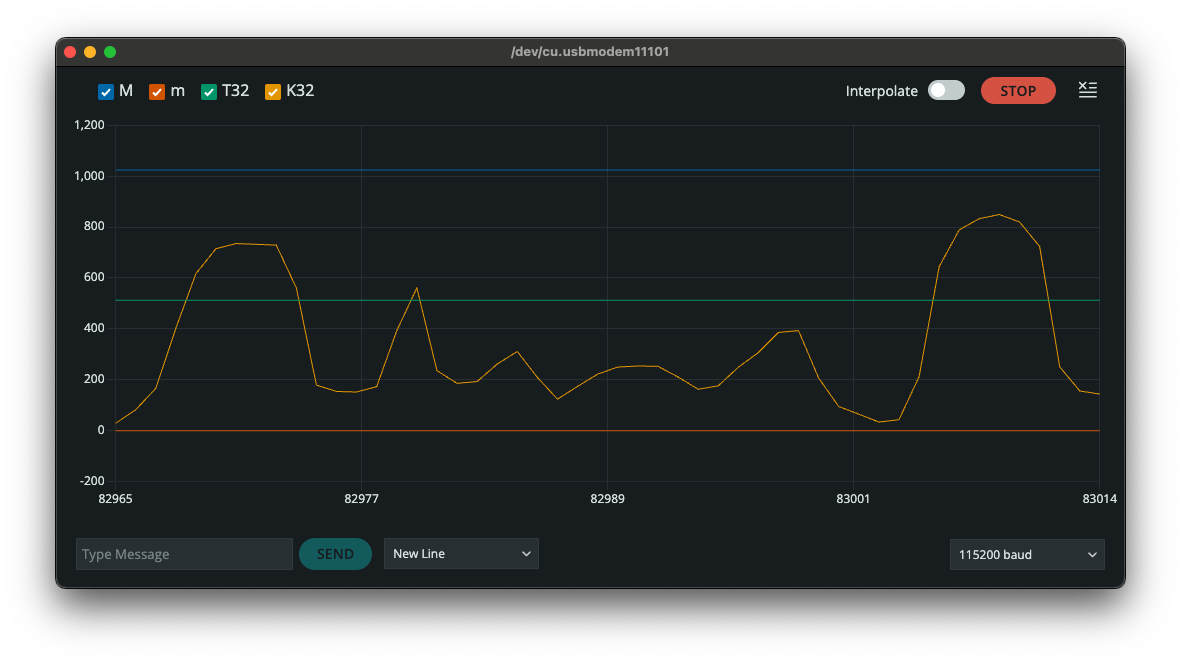
\includegraphics[width=\linewidth]{src/images/serial_monitor.png}
%     \caption{Arduino IDE serial plotter used for calibration of sensor thresholds. \texttt{M} and \texttt{m} represent the maximum an minimum value of digitised data. \texttt{K} and \texttt{T} are the values of the sensor and threshold being calibrated, followed by a two-digit number denoting the sensor index (in this case, sensor 32).}
%     \label{fig:serial_monitor}
% \end{figure}

\subsection{Final Assembly and Integration}

The final 49-key harpsichord replica incorporated the sensor and controller boards into the rectangular frame. Ribbon cables connected the PCBs, while felt strips were interwoven between the strings to suppress vibrations and maintain the tactile response of the keys. The assembly process at the \anon{NEMUS} lab in \anon{Bologna} involved meticulous adjustments to key clearances and wiring layouts. Modifications included milling sections of the keys to ensure adequate clearance for the PCBs and varnishing the jacks to improve sticker adhesion. The sample library, purchased from Spitfire Audio and controlled via Native Instrument's Kontakt, was installed on a Mac Mini hosted inside the instrument's case. Special holes drilled at the back of the instrument's frame, away from sight, allow the passage of cables, such as from power supplies, USB connectors and headphone jack. An iPad is used as the secondary monitor, displaying the library alone. Users interact with the library through it, while the main 12-inch display sits inside a custom-made drawer locked during usage.



\section{Discussion}\label{context}


In an effort to make the exhibition more accessible and authentic, the \anon{San Colombano Museum} commissioned the construction of a mechanical keyboard to trigger a MIDI-controlled sample library, designed for use by museum visitors. The exhibition is set to open approximately a month after this work's submission, and only preliminary feedback has been collected from a pool of testers. The keyboard shows significant promise in enhancing the museum experience. Testers unfamiliar with harpsichords were particularly impressed by its responsiveness. The keyboard is hosted in the \emph{Oratory} above the museum's main hall, an exceptional testimony to the Bolognese art, decorated by the finest students of the Carracci and presenting a series of frescoes covering most of the walls and ceiling. The room hosts unique examples of the Italian Renaissance building tradition, including the 1547 harpsichord and the 1540 spinet by Alessandro Trasuntino. Visitors often visit the room with the same caution and respect that is typical of worship spaces. Testers did not find that the exposed headphones and touchscreen affected such an experience negatively, though a more definitive answer will come as more feedback is collected after launch. Pictures of the keyboard hosted in the \emph{Oratory} are shown in Figure \ref{fig:oratory}.

Expert feedback has highlighted certain limitations, including imprecise key calibration, which creates a temporal disconnect between the tactile plucking sensation and sound onset. Additionally, the commercial sample library, while allowing the selection of registers such as 8', 4', and their combinations, restricts functionality to a single MIDI message per key, regardless of the number of string choirs controlled. Inspired by early Italian instruments, the keyboard's layout is designed to manage two 8' registers. However, one register was disengaged, and sensors were placed before a single set of jacks to accommodate these limitations. Technical improvements, such as refined calibration with hysteresis and developing a custom sample library, could address these constraints in future iterations.

A longer discussion, but one going beyond the scope of this work, is whether the current setup or its future iterations may be effectively used to build legitimate replicas of historical musical instruments or even become a kind of \emph{new} musical instrument altogether. As such, the question is whether these designs may result in music being practised, performed and recorded with the instruments. This work supports an overarching narrative extending beyond its application in museum collections. The \anon{NEMUS project \cite{NEMUS}}, focusing on developing advanced physical models simulating the non-linear interaction between subcomponents, has commissioned a second keyboard to further explore the role of control interfaces in performance, exploiting the inherently bi-directional signal paths linking the mechanical world with the virtual, replicating the embodied relationships between performer and instrument and offering opportunities to modify or even disrupt these interactions. The upcoming Rem@ke project \cite{remake1} has also expressed an interest in engaging with the keyboard to explore meaningful embodied interactions between players and instruments. 


\section{Conclusion}\label{conclusion}

This study has presented the design and implementation of an electronically augmented keyboard for the Tagliavini Collection at the San Colombano Museum. By leveraging optical sensors and MIDI-controlled sample libraries, the keyboard allows users to explore a harpsichord's sonic and mechanical essence without compromising the integrity of the museum's historical artefacts. Preliminary feedback shows that the keyboard has the potential to enhance the museum experience, particularly for those unfamiliar with early keyboard instruments. However, technical limitations, such as calibration inconsistencies and restrictions imposed by the commercial sample library, highlight opportunities for refinement. These issues will be addressed in future iterations, including a second keyboard designed to control advanced physical models. This work opens new possibilities for engaging with heritage collections while respecting their authenticity. It also serves as a foundation for further research projects exploring embodied cognition in historical instruments, and it may provide a useful framework to investigate the links between physical modelling and digital musical interface design.

